\documentclass{article}
\usepackage{graphicx} % Required for inserting images
\usepackage{multicol}
\usepackage[shortlabels]{enumitem}
\usepackage{listings}
\usepackage{xcolor}
\usepackage{inconsolata}

\lstset{
    basicstyle=\ttfamily\color{red},
    language=C++,
}

\title{
Algoritmos e Estrutura de Dados PCO001

Resolução de: \textbf{Exercícios - Fila}
}
\author{Carlos Augusto Ribeiro}
\date{2024-01}

\begin{document}

\maketitle

\par
\noindent
\textbf{Tarefa 1} -  Considere a fila de inteiros F1 da Figura 1. Implemente uma função que remove todos os valores negativos da fila

\begin{figure}[h!]
    \clearpage
    \centering
    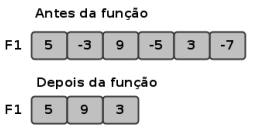
\includegraphics[width=0.5\linewidth]{fila/1.PNG}
    \caption{Fila F1 e o comportamento da função para retirar elementos negativos.}
\end{figure}

\bigskip
\par
\noindent
\textbf{Solução}
\begin{lstlisting}
bool removeNumerosNegativos(Fila &fila) {
    int valor;
    int qtd = 0;
    int tamanhoInicial = fila.Nro;
    while (qtd < tamanhoInicial && RetiraFila(fila, valor)) {
        if (valor > 0) InsereFila(fila, valor);
        qtd++;
    }
    return qtd > fila.Nro;
}
\end{lstlisting}

\bigskip

\par
\noindent
\textbf{Tarefa 2} - Considere as seguintes funções:
\begin{itemize}
    \item \textbf{Enqueue(F, a)}: Aumenta o tamanho da fila \textbf{F}, acrescentando o elemento a no fim da fila (insere na fila);
    \item \textbf{Dequeue(F)}: Remove e retorna o elemento que está no começo da fila F (retira da fila);
\end{itemize}

\par
\noindent
Observe a seguir como estas operações interagem para alterar o estado de uma fila \textbf{F}, inicialmente vazia (\textbf{F[ ]}), cuja extremidade esquerda representa o começo da fila e a extremidade direita o fim. Por exemplo, imagine a fila \textbf{F} com os elementos \textbf{[r, g]}. Ao executar o comando \textbf{Enqueue(F,b)}, a fila F ficaria \textbf{[r,g,b]}.
\begin{enumerate}[(a)]
    \item Enqueue(F,a); \( \rightarrow \) \textcolor{red}{[a]}
    \item Enqueue(F,Dequeue(F)); \( \rightarrow \) \textcolor{red}{[a]}
    \item Enqueue(F,b); \( \rightarrow \) \textcolor{red}{[a,b]}
    \item Dequeue(F); \( \rightarrow \) \textcolor{red}{[b]}
    \item Enqueue(F,c); \( \rightarrow \) \textcolor{red}{[b,c]}
    \item Enqueue(F,e); \( \rightarrow \) \textcolor{red}{[b,c,e]}
    \item Dequeue(F); \( \rightarrow \) \textcolor{red}{[c,e]}
\end{enumerate}

\bigskip

\par
\noindent
\textbf{Tarefa 3} - Considere uma fila \textbf{F} de valores inteiros. Implemente uma função que calcula a média dos valores contidos em \textbf{F} (Figura 2).
\begin{figure}[h!]
    \clearpage
    \centering
    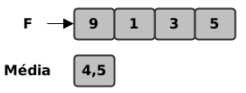
\includegraphics[width=0.5\linewidth]{fila/2.PNG}
    \caption{ Fila F e o resultado da função que calcula a média do valores contidos em F.}
\end{figure}

\bigskip
\par
\noindent
\textbf{Solução}
\begin{lstlisting}
double mediaFila(Fila &fila) {
    if (fila.Nro == 0) return 0;
    double sum = 0;
    int valor;
    int qtd = 0;
    int tamanhoInicial = fila.Nro;
    while (qtd < tamanhoInicial && RetiraFila(fila, valor)) {
        sum+=valor;
        qtd++;
        InsereFila(fila, valor);
    }
    return sum / fila.Nro;
}
\end{lstlisting}

\bigskip

\par
\noindent
\textbf{Tarefa 4} -  Considere uma fila \textbf{F} de valores inteiros. Implemente uma função que retorna o menor elemento desta fila.\\
\textbf{Protótipo}: int MenorFila(Fila \&F);
\bigskip
\par
\noindent
\textbf{Solução}
\begin{lstlisting}
int MenorFila(Fila &fila) {
    if (fila.Nro == 0) return 0;
    int valor;
    int menor;
    int qtd = 0;
    int tamanhoInicial = fila.Nro;
    while (qtd < tamanhoInicial && RetiraFila(fila, valor)) {
        if (qtd == 0 || valor < menor) menor = valor;
        qtd++;
        InsereFila(fila, valor);
    }
    return menor;
}
\end{lstlisting}

\bigskip

\par
\noindent
\textbf{Tarefa 5} - Considere uma fila F de valores inteiros. Implemente uma função que inverta a ordem dos elementos desta fila.\\
\textbf{Protótipo}: void InverteFila(Fila \&F)
\bigskip
\par
\noindent
\textbf{Solução}
\begin{lstlisting}
void InverteFila(Fila &fila) {
    if (!FilaVazia(fila)) {
        int valor;
        RetiraFila(fila, valor);
        InverteFila(fila);
        InsereFila(fila, valor);
    }
}
\end{lstlisting}
\end{document}
